%!TEX program = lualatex 
%!TEX encoding = UTF-8 Unicode  
%!TEX root = chapter07.tex  
\documentclass[main.tex]{subfiles} 
\begin{document} 
%----------------------------------------------------------------------------------------
%	CHAPTER 7
%----------------------------------------------------------------------------------------
\newpage 
\loadgeometry{marginlayout}  
\pagestyle{scrheadings} % Print headers again  
\KOMAoptions{
	headwidth=textwithmarginpar,
	headsepline=true,
	headsepline= 0.5pt,
	footwidth=textwithmarginpar,
}  
\onehalfspacing 
\setcounter{chapter}{6}

\chapter{Variables aléatoires finies}
Soit une expérience aléatoire d'univers $\Omega=\{ \omega_1, \omega_2, \ldots , \omega_N\}$  et sa   loi de probabilité $P$.

\begin{definition} Une variable aléatoire $X$ est une fonction 
	\setlength{\abovedisplayskip}{3pt}
	\setlength{\belowdisplayskip}{3pt}  
$$X\colon \begin{aligned}[t] \Omega &\to \mathbb{R}\\
		\omega & \mapsto X(\omega)=x
	\end{aligned}$$
 $X(\Omega)=\{x_1; x_2; \ldots ; x_n\}$  l'ensemble des images possibles.\\
Pour $x\in\mathbb{R}$ on note : \sidenote{la partie de $\Omega$ des issues $\omega$ pour lesquelles $X(\omega)=x$}
\setlength{\abovedisplayskip}{3pt}
\setlength{\belowdisplayskip}{3pt}  
$$\{X=x\}=\{\omega\in\Omega ~|~ X(\omega)=x\}$$ 
On pose :\sidenote{somme des probabilités des issues qui ont pour image $x$}
\setlength{\abovedisplayskip}{3pt}
\setlength{\belowdisplayskip}{3pt}  
$$
P(X=x)= \sum_{\omega ~|~ X(\omega)=x} p(\omega) 
$$
\end{definition}  
\begin{example} \label{chapter07:example01}
On considère le jeu suivant : \og On lance un dé cubique équilibré et on note la face obtenue. \fg{}. 
\begin{enumerate}[label={\textbullet}, leftmargin=*] 
	\item Si le résultat est pair, on gagne $2$\euro. 
	\item Si le résultat est $1$, on gagne $4$\euro. 
	\item Si le résultat est $3$ ou $5$, on perd $4$\euro.
\end{enumerate}
L'univers est $\Omega= \left\lbrace 1; 2; 3; 4; 5; 6 \right\rbrace$ avec les issues $1$ à $6$ équiprobables. $X$  est la variable aléatoire des gains.

\vspace{-0.5em}	  
\begin{spacing}{2}
	\begin{enumerate}[label={}, leftmargin=*] 
		\item $X(1)=\dotfill$ $X(4)=\dotfill$  $X(5)=\dotfill$  $X(6)=\dotfill$ 
		\item $\{ X = 2\}=\{\dotfill  \}$ \hfill   $\{ X = -4\}=\{\dotfill  \}$ \hfill $\{ X = 4\}= $ 
		\item $P(X=2)=$\dotfill $P(X=-4)=$\dotfill $P(X=4)=$  
		\item On résume les probabilités précédentes  sous forme de tableau : \\
			\renewcommand{\arraystretch}{1.1} 
		\null	\hfill \begin{tabularx}{0.7\linewidth}{|c|Y|Y|Y|c|}
				\hline
				\cellcolor{blue!10}{$x_i$} & $-4$ & $2$ & $4$ & \textbf{Total}\\ \hline
				\cellcolor{blue!10}{$P(X=x_i)$} &  &   &   & \\\hline
			\end{tabularx}  
			\hfill\null
			\smallskip
		\item $\{ X \geqslant -4\}=\{\dotfill  \}$ \hfill $P(X\geqslant -4)=$
		\item $\{0 < X \leqslant \numprint{4.5}\}=\{\dotfill  \}$\hfill $P(0 < X \leqslant \numprint{4.5})=$
	\end{enumerate}
\end{spacing}  \vspace{-0.75em}	   
 
\end{example}
 

\begin{definition}[]  $X$ v.a. réelle finie, prenant les valeurs $x_1; \ldots ; x_n$. La \textbf{loi de probabilité de la variable $X$} est la   probabilité $P_X$ définie sur \emph{des} parties de $I\subset \mathbb{R}$ :\sidenote{typiquement des singletons $\{x\}$ ou des intervalles}  
	\setlength{\abovedisplayskip}{3pt}
	\setlength{\belowdisplayskip}{3pt}  
$$
P_X(I)=P(X\in I)=\sum_{x_i\in I} P(X=x_i)
$$ 
En particulier $P(X\in\mathbb{R})=\sum_{i=1}^n P(X=x_i)=1$.
\end{definition}
\begin{definition}  $X$ v.a. réelle finie, prenant les valeurs $x_1; \ldots ; x_n$. L'\textbf{espérance de $X$} est le réel noté $\Expect{X}$ :  
	\setlength{\abovedisplayskip}{3pt}
	\setlength{\belowdisplayskip}{3pt}  
	$$
	\mu = \Expect{X}=\sum_{x\in\mathbb{R}} xP(X=x) = \sum_{i=1}^{n} x_i P(X=x_i)
	$$ 
\end{definition}
\begin{example} En reprenant la v.a. de l'exemple \ref{chapter07:example01}, on a :
	\setlength{\abovedisplayskip}{3pt}
	\setlength{\belowdisplayskip}{3pt}  
	\[
	\Expect{X}=\sum x_iP(x=x_i)  = (-4)\times \qquad + 2\times \qquad + 4\times \qquad = \frac{1}{3}
	\]
\end{example}
\begin{remark}  On repète une expérience aléatoire un nombre $N$ \textbf{assez grand} de fois. On enregistre les valeurs obtenues de la v.a. $X$. 
$\Expect{X}$ approche la moyenne des valeurs observées sur les $N$ répétitions.
\end{remark}
\begin{proof} 	Pour tout $i$, on note $n_i=$ le nombre d'observation de la valeur $x_i$ durant les $N$ répétitions. La loi des grands nombres dit que :
	\setlength{\abovedisplayskip}{3pt}
	\setlength{\belowdisplayskip}{3pt}  
	\begin{align*}
		\forall i& \qquad   P(X=x_i)\approx \frac{n_i}{N}  \\ 
		\Expect{X}&=\sum_i x_iP(X=x_i)\approx \sum_i \left(x_i\frac{n_i}{N}\right) =\frac{ \sum\limits_i n_ix_i }{N}
	\end{align*}
\end{proof}
\begin{definition} $X$ v.a. réelle finie, prenant les valeurs $x_1; \ldots ; x_n$. La \textbf{variance de $X$} est le réel \textbf{positif ou nul} noté $\Var{X}$  :   
	\setlength{\abovedisplayskip}{3pt}
	\setlength{\belowdisplayskip}{3pt}  
	$$	
		\sigma^2 = \Var{X}   =\Expect{(X-\mu)^2}   =  \sum_{i=1}^{n} (x_i-\mu)^2 P(X=x_i)
	$$
	L'\textbf{écart-type} $\sigma=\sqrt{\Var{X}}$ est l'\emph{écart quadratique moyen à $\mu$}.
\end{definition}
\begin{remark} L'écart-type est une mesure de la dispersion de la v.a. autour de la moyenne. Plus l'écart-type est petit, plus la variable aléatoire est centrée autour de sa moyenne. Plus précisément, l'\textbf{inégalité de Tchebychev} \sidenote{vue en terminale}  :
	\setlength{\abovedisplayskip}{3pt}
	\setlength{\belowdisplayskip}{3pt}  
	$$	
	P(\abs{X-\mu}\geqslant k\sigma ) \leqslant \frac{1}{k^2}
	$$ 
En particulier :
	\begin{align*}
		P(-2\sigma< X-\mu<2\sigma )& \geqslant 75\%\\
		P(-5\sigma< X-\mu<5\sigma )& \geqslant 96\%
	\end{align*}

\end{remark}
%\begin{proof}
%	La démonstration de ce résultat est simple.
%	\setlength{\abovedisplayskip}{3pt}
%	\setlength{\belowdisplayskip}{3pt}  
%	$$
%	\sigma^2=\sum_{i=1}^n (x_i-\mu)^2 P(X=x_i)
%	\geqslant \sum_{\abs{x_i-\mu}>k\sigma }^n (x_i-\mu)^2 P(X=x_i) 
%	\geqslant k^2\sigma^2\sum _{\abs{x_i-\mu}>k\sigma }^n  = P(\abs{x_i-\mu}>k\sigma)
%	$$
%\end{proof} 
%----------------------------------------------------------------------------------------
%	 
%----------------------------------------------------------------------------------------
\newpage 
\loadgeometry{widelayout}  
\pagestyle{scrheadings} % Print headers again  
\KOMAoptions{
	headwidth=textwithmarginpar,
	headsepline=true,
	headsepline= 0.5pt,
	footwidth=textwithmarginpar,
}  
\onehalfspacing 
\section{Exercices variables aléatoires finies et indicateurs}

\begin{exercise}
	Une tombola comporte 100 tickets et un unique ticket gagnant permettant de remporter \EUR{10000}.
	

\begin{spacing}{2} 
\begin{enumerate}[leftmargin=*,label=\arabic*)]
		\item On achète le 3\ieme ticket mis en vente, et on note $X_3$ le gain obtenu.
	\begin{enumerate}[leftmargin=*,label=\alph*)]
		\item Compléter afin de déterminer la loi de probabilité de $X_3$. 
		\begin{enumerate}[leftmargin=*,label={}]   
			\item  La variable aléatoire $X_3$ peut prendre les valeurs   \dotfill  
			\item  Si le ticket tiré est le ticket gagnant alors $X_3 =10000$ et $P(X_3 = 10000) = \dotfill $.
			\item Si le ticket tiré n'est pas gagnant alors $X_3=0$ et $P(X_3=0)=$\dotfill 
		\end{enumerate}
		\item Compléter le tableau définissant la loi de probabilité de $X_3$ :\\
		\renewcommand{\arraystretch}{1.0} 
		\null	\hfill \begin{tabularx}{0.7\linewidth}{|c|Y|Y|Y|}
			\hline
			\cellcolor{blue!10}{$x$} & $0$ & $10000$  & \textbf{Total} \\ \hline
			\cellcolor{blue!10}{$P(X_3=x)$} &   &  & \\\hline
		\end{tabularx} 
		\hfill \null\medskip
		\item  $\Expect{X_3}=\sum_{i=1}^2 x_iP(X_3=x_i) = 0\times\qquad +\numprint{10000}\times \qquad  = $\dotfill  
	\end{enumerate}
	\item  On achète le 3\ieme ticket mis en vente puis le 57\ieme. On note $X_3$ et $X_{57}$ les V.A. des gains de chaque ticket. On note $Y=X_3+X_{57}$ le gain total.
	\begin{enumerate}[leftmargin=*,label=\alph*)]
		\item Complétez et justifier que les événements $A=\{X_3=0\}$ et $B=\{X_{57}=0\}$ ne sont pas indépendants :\\
		$P(B)=$\dotfill ; ~$P_A(B)=$ \dotfill ; ~ On a \dotfill\dotfill\dotfill  
		\item Compléter afin de déterminer la loi de probabilité de $Y$. 
		\begin{enumerate}[leftmargin=*,label={}]   
			\item  La variable aléatoire $Y$ peut prendre les valeurs   \dotfill  
			\item  Si  le ticket gagnant est parmi les tickets achetés alors $Y =10000$ et $P(Y = 10000) = \dotfill $.
			\item Si  le ticket gagnant n'est pas parmi les tickets achetés $Y=0$ et $P(Y=0)=$\dotfill 
		\end{enumerate}
		\item Compléter le tableau définissant la loi de probabilité de $Y$ :\\
		\renewcommand{\arraystretch}{1.0} 
		\null	\hfill \begin{tabularx}{0.7\linewidth}{|c|Y|Y|Y|}
			\hline
			\cellcolor{blue!10}{$y$} & $0$ & $10000$ &  \textbf{Total} \\ \hline
			\cellcolor{blue!10}{$P(Y=y)$} &   &  & \\\hline
		\end{tabularx} 
		\hfill \null\smallskip
		\item  $\Expect{Y}=\sum_{i=1}^2 x_iP(X=x_i) = 0\times\qquad +\numprint{10000}\times \qquad  = $\dotfill 
		\item On constate que $\Expect{Y}= \Expect{X_3+X_{57}}=$\dotfill 
	\end{enumerate} 
	\item $Z$ est la V.A. des gains lorsque l'on achète les 100 tickets. $\Expect{Z}=$\dotfill 
\end{enumerate}
\end{spacing} 
\vspace{-0.5em} 
\end{exercise}
% parler de si on achète 100 tickets ? 
\begin{exercise}  On tire au hasard successivement 3 cartes numérotées de 1 à 3 et on note les valeurs des cartes dans l'ordre d'apparition. La V.A. $X$ désigne le nombre carte dont la valeur est égale à son rang.\\
	\null\hfill 
	\begin{tikzpicture}[xscale=1,yscale=1]
		% Styles (MODIFIABLES)
		\tikzstyle{fleche}=[-,>=latex,thick]
		\tikzstyle{noeud}=[rounded corners=5pt]
		\tikzstyle{feuille}=[]
		\tikzstyle{commentaire}=[black]
		% Dimensions (MODIFIABLES)
		\def\DistanceInterNiveaux{3}
		\def\DistanceInterFeuilles{1.25}
		% Dimensions calculées (NON MODIFIABLES)
		\def\NiveauA{(0)*\DistanceInterNiveaux}
		\def\NiveauB{(0.50)*\DistanceInterNiveaux}
		\def\NiveauC{(1.5)*\DistanceInterNiveaux}
		\def\NiveauD{(2.250)*\DistanceInterNiveaux}
		\def\NiveauE{(3.0)*\DistanceInterNiveaux}
		\def\NiveauF{(3.75)*\DistanceInterNiveaux}
		\def\InterFeuilles{(-1)*\DistanceInterFeuilles}
		% Noeuds (MODIFIABLES : Styles et Coefficients d'InterFeuilles)
		\node[commentaire] (epreuve1) at ({\NiveauB},{(0)*\InterFeuilles}) {\scriptsize rang \no 1};
		\node[commentaire] (epreuve2) at ({\NiveauC},{(0)*\InterFeuilles}) {\scriptsize rang \no 2}; 
		\node[commentaire] (epreuve3) at ({\NiveauD},{(0)*\InterFeuilles}) {\scriptsize rang \no 3};
		\node[commentaire] (issues) at ({\NiveauE},{(0)*\InterFeuilles}) {\scriptsize issues};
		\node[commentaire] (va) at ({\NiveauF},{(0)*\InterFeuilles}) {\scriptsize  valeurs de $X$};
		% 
		\node[noeud] (R) at ({\NiveauA},{(3.5)*\InterFeuilles}) {};
		\node[noeud] (Ra) at ({\NiveauB},{(1.5)*\InterFeuilles}) {1};
		\node[feuille] (Raa) at ({\NiveauC},{(0.5)*\InterFeuilles}) {2};  
		\node[feuille] (Raaa) at ({\NiveauD},{(0.5)*\InterFeuilles}) {3}; 
		\node[feuille] (Rab) at ({\NiveauC},{(2)*\InterFeuilles}) { }; 
		\node[noeud] (Rb) at ({\NiveauB},{(3.5)*\InterFeuilles}) { };
		\node[feuille] (Rba) at ({\NiveauC},{(3)*\InterFeuilles}) { }; 
		\node[feuille] (Rbb) at ({\NiveauC},{(4)*\InterFeuilles}) { }; 
		\node[noeud] (Rc) at ({\NiveauB},{(5.5)*\InterFeuilles}) { };
		\node[feuille] (Rca) at ({\NiveauC},{(5)*\InterFeuilles}) { }; 
		\node[feuille] (Rcb) at ({\NiveauC},{(6)*\InterFeuilles}) { }; 
		%
		\node[commentaire] (I1) at ({\NiveauE},{(0.5)*\InterFeuilles}) {\AffCarteJeu[Hauteur=1,Tikz]{AC}
			\AffCarteJeu[Hauteur=1,Tikz]{2C}
			\AffCarteJeu[Hauteur=1,Tikz]{3C}  }; 
		%	\node[commentaire] (I2) at ({\NiveauD},{(1.5)*\InterFeuilles}) {$A\cap \overline{B}$}; 
		%	\node[commentaire] (I3) at ({\NiveauD},{(2.25)*\InterFeuilles}) {$\overline{A}\cap B$}; 
		%	\node[commentaire] (I4) at ({\NiveauD},{(3.25)*\InterFeuilles}) {$\overline{A}\cap \overline{B}$};
		%	%
		\node[commentaire] (P1) at ({\NiveauF},{(0.5)*\InterFeuilles}) {$X=3$}; 
		%	\node[commentaire] (P2) at ({\NiveauE},{(1.5)*\InterFeuilles}){$P(A\cap \overline{B})= $}; 
		%	%	\draw (P2.east) node[anchor=west, commentaire] {Faux négatif};
		%	\node[commentaire] (P3) at ({\NiveauE},{(2.25)*\InterFeuilles}){$P(\overline{A}\cap B)= $}; 
		%	%	\draw (P3.east) node[anchor=west, commentaire] {Faux positif};
		%	\node[commentaire] (P4) at ({\NiveauE},{(3.25)*\InterFeuilles}) {$P(\overline{A}\cap \overline{B})=$}; 
		%	%		\draw[ ultra thick] ({\NiveauE-1},{(3.55)*\InterFeuilles}) -- ({\NiveauE+1},{(3.55)*\InterFeuilles}) ;
		%	%		\node[commentaire] (P5) at ({\NiveauE},{(3.75)*\InterFeuilles})  {\textbf{Total}$=\ldots $}; 
		%	
		% Arcs (MODIFIABLES : Styles)
		\draw[fleche] (R.east)--(Ra.west) node[midway, above]{ };
		\draw[fleche] (Ra.east)--(Raa.west) node[midway, above]{ };
		\draw[fleche] (Raa.east)--(Raaa.west) node[midway, above]{ };
		%		\draw[fleche] (Ra.east)--(Rab.west) node[midway, below]{};
		\draw[fleche] (R.east)--(Rb.west) node[midway, above]{};
		%		\draw[fleche] (Rb.east)--(Rba.west) node[midway, above]{};
		%		\draw[fleche] (Rb.east)--(Rbb.west) node[midway, below]{};
		\draw[fleche] (R.east)--(Rc.west) node[midway, below]{};
		%		\draw[fleche] (Rc.east)--(Rca.west) node[midway, above]{};
		%		\draw[fleche] (Rc.east)--(Rcb.west) node[midway, below]{};
	\end{tikzpicture} 
	\hfill \null  
	
	\begin{spacing}{1.7} 
		\begin{enumerate}[leftmargin=*,label={\arabic*)}]
			\item Compléter l'arbre ci-dessous 
			\item Compléter le tableau définissant la loi de probabilité de $X$ \\
			\renewcommand{\arraystretch}{1.0} 
			\null	\hfill \begin{tabularx}{0.7\linewidth}{|c|Y|Y|Y|Y|Y|}
				\hline
				\cellcolor{blue!10}{$x$} & $0$ & $1$ & $2$ &$3$ & \textbf{Total} \\ \hline
				\cellcolor{blue!10}{$P(X=x)$} &   &  &   &   & \\\hline
			\end{tabularx} 
			\hfill \null\medskip 
		\item	$\Expect{X}=0\times P(X=0)+\ldots\times P(X=\ldots)+\ldots\times P(X=\ldots) +\ldots\times P(X=\ldots) $  \\
	\null	$\Expect{X}=$\dotfill  
		\end{enumerate}\vspace{-1em}
	\end{spacing}
\end{exercise} 
\begin{exercise} On lance deux dés  (d4) équilibrés. On note $M$ la variable aléatoire correspondant au maximum, et $S$ la somme des deux valeurs obtenues. À l'aide des diagrammes double entrée, déterminer les loies de probabilité de $M$ et $S$ et leur espérances.\\
		\noindent  
		\parbox{0.65\linewidth}{
\begin{spacing}{2}
		 \renewcommand{\arraystretch}{1.0} 
 	\begin{enumerate}[leftmargin=*,label=\arabic*)]
 	\item 
		 \null	\hfill \begin{tabularx}{1\linewidth}{|c|Y|Y|Y|Y|c|}
		 	\hline
		 	\cellcolor{blue!10}{$x$} & $1$ & $2$ & $3$ &$4$ & \textbf{Total} \\ \hline
		 	\cellcolor{blue!10}{$P(M=x)$} &   &  &   &   & \\\hline
		 \end{tabularx}  \smallskip \\
	 \null	\hfill \begin{tabularx}{1\linewidth}{|c|Y|Y|Y|Y|Y|Y|Y|c|}
	 	\hline
	 	\cellcolor{blue!10}{$x$} & $~$ & $~$ & $~$ &$~$ & $~$ & $~$ & $~$ & \textbf{Total} \\ \hline
	 	\cellcolor{blue!10}{$P(S=x)$} &   &  &   &   & & & & \\\hline
	 \end{tabularx}  \smallskip
	 \item  $\Expect{M}=$\dotfill \\
	 \null\dotfill
	 \item  $\Expect{S}=$\dotfill \\
	 \null\dotfill
\end{enumerate}
\end{spacing}
		}
		\parbox{0.3\linewidth}{ 
		\begin{tabular}{|*2{c|}*4{c}|}
			\cline{3-6}
			\multicolumn{2}{c|}{\multirow{2}{*}{}} & \multicolumn{4}{c|}{Dé \no 2}  \\ \cline{3-6}
			\multicolumn{2}{c|}{}   &   \rule{0em}{1.2em}$\quad$ &   $\quad$  & $\quad$  &  $\quad$  \\ \hline
			\multirow{4}{*}{\rotatebox[origin=c]{90}{Dé \no 1}}	
			&  $\quad$  &  \rule{0em}{1.3em} &   &  &     \\ %\cline{2-6}
			&  $\quad$ & \rule{0pt}{1.3em}\rule{1.3em}{0em}  &  \rule{1.3em}{0em}  &  \rule{1.3em}{0em}&\rule{1.3em}{0em}  \\ %\cline{2-6}
			&  $\quad$ & \rule{0pt}{1.5em}\rule{1.3em}{0em}  &  \rule{1.3em}{0em}  &  \rule{1.8em}{0em}&\rule{1.3em}{0em}  \\ %\cline{2-6} 
			& $\quad$  &  \rule{0pt}{1.3em} &   &  &      \\ \hline
		\end{tabular}   \\
		\begin{tabular}{|*2{c|}*4{c}|}
			\cline{3-6}
			\multicolumn{2}{c|}{\multirow{2}{*}{}} & \multicolumn{4}{c|}{Dé \no 2}  \\ \cline{3-6}
			\multicolumn{2}{c|}{}   &   \rule{0em}{1.2em}$\quad$ &   $\quad$  & $\quad$  &  $\quad$  \\ \hline
			\multirow{4}{*}{\rotatebox[origin=c]{90}{Dé \no 1}}	
			&  $\qquad$  &  \rule{0em}{1.3em} &   &  &     \\ %\cline{2-6}
			&  $\qquad$ & \rule{0pt}{1.3em}\rule{1.3em}{0em}  &  \rule{1.3em}{0em}  &  \rule{1.3em}{0em}&\rule{1.3em}{0em}  \\ %\cline{2-6}
			&  $\qquad$ & \rule{0pt}{1.5em}\rule{1.3em}{0em}  &  \rule{1.3em}{0em}  &  \rule{1.8em}{0em}&\rule{1.3em}{0em}  \\ %\cline{2-6} 
			& $\qquad$  &  \rule{0pt}{1.3em} &   &  &      \\ \hline
		\end{tabular} 
		} 
\end{exercise}
  
\begin{exercise} Soit l'expérience aléatoire \og on tire une carte dans un jeu de 32 cartes \fg et le jeu suivant : \hfill \\
\noindent
\parbox{0.65\linewidth}{ 
	\begin{enumerate}[leftmargin=*,label=\textbullet]
		\item  Si on tire un coeur, on gagne $2$\euro.
		\item  Si on tire un roi, on gagne $5$\euro.
		\item  Si on tire une autre carte, on perd $1$\euro.
\end{enumerate}
}
\hfill  
\parbox{0.3\linewidth}{
\MainMiniCartesJeu[Hauteur=2,]{A.C § R.C § D.C § V.C § 10.C § 9.C§ 8.C§ 7.C} \\
\MainMiniCartesJeu{A.K § R.K § D.K § V.K § 10.K § 9.C§ 8.K§ 7.K} \\
\MainMiniCartesJeu{A.T § R.T § D.T § V.T § 10.T § 9.T§ 8.T§ 7.T} \\
\MainMiniCartesJeu{A.P § R.P § D.P § V.P § 10.P § 9.P§ 8.P§ 7.P} 	
}\medskip\\ 
On appelle $X$ la variable aléatoire qui à une carte associe le gain (ou la perte).
\vspace{-0.25em}
\begin{spacing}{2} 
\begin{enumerate}[leftmargin=*,label=\arabic*)]
	\item Compléter afin de déterminer la loi de probabilité de $X$. 
\begin{enumerate}[leftmargin=*,label={}]   
	\item  La variable aléatoire $X$ peut prendre les valeurs $-1$, $2$, $5$ et \dotfill  
	\item  Si la carte tirée est le roi de coeur \AffMiniCarteJeu{R.C}, on gagne, $X =\ldots+ \ldots=7$ et $P(X = 7) = \dotfill $.
	\item  Si la carte tirée est un coeur (mais pas un roi), $X = \dotfill $ et $P(X = \ldots) = \dotfill$.
	\item  Si la carte tirée est un roi (mais pas un coeur), $X = \dotfill $ et $P(X = \ldots) = \dotfill$.
	\item  Si la carte tirée n'est ni un coeur, ni un roi, $X = \dotfill $ et $P(X = \ldots) = \dotfill$.
	\end{enumerate}
\item Compléter le tableau définissant la loi de probabilité de $X$ :\\
\renewcommand{\arraystretch}{1.1} 
\null	\hfill \begin{tabularx}{0.7\linewidth}{|c|Y|Y|Y|Y|Y|}
	\hline
	\cellcolor{blue!10}{$x$} & $-1$ & $2$ & $5$ & $\qquad$ & \textbf{Total} \\ \hline
	\cellcolor{blue!10}{$P(X=x)$} &   &   &    &  &   \\\hline
\end{tabularx} 
\hfill \null\medskip
\item $P(X\geqslant 5)=P(X=\ldots\ldots)+P(X=\ldots\ldots)=$\dotfill  \\
La probabilité de \dotfill est égale à $\frac{1}{8}$.\\
Dans 1000 répétitions de l'expérience, les gains dépassent 5 \euro~ dans   $1000 \times\phantom{ P(X\geqslant 5)} \approx \dotfill $ des essais. 
\item $\Expect{X}=\sum_{i=1}^4 x_iP(X=x_i) = -1\times\qquad +2\times \qquad +5\times \qquad + 7\times \qquad = $\dotfill \\ 
Dans 1000 répétitions de l'expérience, le total des gains $\approx 1000\times \dotfill =\dotfill $\euro
\end{enumerate}\vspace{-1.5em}
\end{spacing}  
\end{exercise} 
\begin{exercise} 
	On fait tourner l'aiguille et on note la valeur $X$ du gain obtenu. \\ 
	\vspace{-1.5em}
	\noindent
	\begin{spacing}{2} 
\begin{enumerate}[leftmargin=*,label=\arabic*)]
			\item 
		Identifier les issues et compléter le tableau de la loi de probabilité de la v.a. $X$.\\
	\noindent	
\parbox{0.80\linewidth}{
	\hfill \null 
		\renewcommand{\arraystretch}{1.0} 
		\null	\hfill \begin{tabularx}{0.9\linewidth}{|c|Y|Y|Y|}
			\hline
			\cellcolor{blue!10}{$x$ en \euro} &   &   &       \\ \hline
			\cellcolor{blue!10}{$P(X=x)$} & &    &        \\\hline
		\end{tabularx} 
	}
\hfill 
\parbox[position=t]{0.2\linewidth}{ \centering
\noindent
\hfill
\begin{tikzpicture}[scale=0.6]
	\tkzSetUpPoint[size=2, fill=black]
	\tkzfctset{tan style/.style={->,>=latex, color=red, line width=1.2pt}}   
	\tkzSetUpLine[line width= 1.2pt, add=.5 and .5]  
	%			\tkzInit[xmin=-1.0,ymin=-1.0,xmax=6.5,ymax=2.8]
	%			\tkzClip
	
	\def\a{2.0}
	\tkzDefPoint(0,0){O} 
	
	\foreach \x [count = \xi] in {0,120,240}
	{
		\tkzDefShiftPoint[O](\x:\a){A\xi}
	} 
	\tkzFillSector[draw,line width=1.2pt,fill=white, ](O,A1)(A2)
	\tkzFillSector[draw,line width=1.2pt,fill=white](O,A2)(A3)
	\tkzFillSector[draw,line width=1.2pt,fill=white,](O,A3)(A1)   
	\tkzText[](60:1.25){$5$~\euro} 
	\tkzText[](180:1.25){$10$~\euro} 
	\tkzText[](-90:1.25){$20$~\euro}
	\tkzDefPoint(1,-0.5){A}
	\tkzDefPoint(-1.5,0.75){B}
	\tkzDrawSegment[line width=1.2pt, |->, >=latex,fill=black, draw=black](A,B) 
\end{tikzpicture}
} 
		\item Déterminer l'espérance du gain $\Expect{X}$.\\
		$\Expect{X}=$\dotfill
		\item Quel est le gain espéré par épreuve lorsqu'on prend compte de la participation de 15 \euro~ par tirage ?
		\end{enumerate}
	\end{spacing} 
\end{exercise}  

\begin{exercise}\label{chapter07:wims:union05} $X$ est la v.a. des gains possibles à une loterie sans tenir compte du prix du billet  :\\
	\renewcommand{\arraystretch}{1.35} 
	\null	\hfill \begin{tabularx}{0.7\linewidth}{|c|Y|Y|Y|Y|Y|}
		\hline
		\cellcolor{blue!10}{$x$ en \euro} & $0$ & $5$ & $10$ & $100$ & $500$ \\ \hline
		\cellcolor{blue!10}{$P(X=x)$} & $\tfrac{4}{20}$ & $\tfrac{4}{20}$  & $\tfrac{10}{20}$  & $\tfrac{1}{20}$& $\tfrac{1}{20}$ \\\hline
	\end{tabularx} 
\hfill \null 
	\begin{spacing}{2} 
	\begin{enumerate}[leftmargin=*,label=\arabic*)]
		\item Déterminer la probabilité de chacun des événements suivants : 
	\begin{enumerate}[leftmargin=*,label={}]
			\item $A=$\og le joueur est gagnant\fg. \hfill $P(A)=P(X>\ldots\ldots)=$\dotfill
			\item $B=$\og le joueur a gagné au moins 100 \euro \fg.
			\hfill
			 $P(B)=P(X\geqslant \ldots\ldots)=$
			 \dotfill
			\item $C=$\og le joueur a gagné au plus 10 \euro \fg.
			\hfill
			 $P(B)=P(X\leqslant \ldots\ldots)=$
			 \dotfill 
			\item $P(A\cap C)=$\dotfill 
		\end{enumerate}
		\item Calculer l'espérance du gain $\Expect{X}$ :\\
		$\Expect{X}=\sum_{i=1}^4 x_iP(X=x_i) =$\dotfill 
		\item L'organisateur pense fixer la participation à 20 \euro. Le jeu sera-t-il favorable au joueur ?
	\end{enumerate} 
\end{spacing} 
\vspace{-0.5em}
\end{exercise} 
\begin{eBox}
En jeu de paris, l'espérence des gains est l'espérence des dividendes attendus moins le taux de participation du jeu. Un jeu est équitable si l'espérence des gains est nulle. 
\end{eBox}  
\begin{exercise} On considère le jeu de hasard. La loi de probabilité de la variable aléatoire $X$ correspondant au gain est résumée dans le tableau :\\
	\renewcommand{\arraystretch}{1.25} 
	\null	\hfill \begin{tabularx}{0.7\linewidth}{|c|Y|Y|Y|Y|}
		\hline
		\cellcolor{blue!10}{$x$} & $0$ & $3$ & $5$ & $50$ \\ \hline
		\cellcolor{blue!10}{$P(X=x)$} & $0.4$ & $0.3$  & $0.28$  & $0.02$  \\\hline
	\end{tabularx} 
	\hfill \null\\
Sachant que le montant de la mise est fixé à \EUR{4}, déterminer si le jeu est équitable.
\end{exercise}
\begin{exercise}
	La loi de probabilité de la variable aléatoire $X$ est donnée dans le tableau ci-dessous :\\
	\renewcommand{\arraystretch}{1.25} 
	\null	\hfill \begin{tabularx}{0.7\linewidth}{|c|Y|Y|Y|Y|Y|}
		\hline
		\cellcolor{blue!10}{$x$} & $1$ & $2$ & $3$ & $4$ & $5$ \\ \hline
		\cellcolor{blue!10}{$P(X=x)$} & $k$ & $2k$  & $4k$  & $2k$& $k$ \\\hline
	\end{tabularx} 
	\hfill \null
	\begin{enumerate}[leftmargin=*,label=\arabic*)]
		\item Donner une équation vérifiée par $k$ et en déduire $k$
		\item En déduire $\Expect{X}$.
		\item On repète l'expérience 1000 fois, et on note les valeurs de $X$ observées.
		\begin{enumerate}
			\item Donner une estimation du nombre d'observations de l'événement $\{X=1\}$
			\item Donner une estimation de la somme des observations.
		\end{enumerate}
	\end{enumerate} 
\end{exercise} 
\begin{exercise}
	La loi de probabilité de la variable aléatoire $X$ est donnée dans le tableau ci-dessous :\\
	\renewcommand{\arraystretch}{1.2} 
	\null	\hfill \begin{tabularx}{0.7\linewidth}{|c|Y|Y|Y|Y|Y|}
		\hline
		\cellcolor{blue!10}{$x$} & $10$ & $20$ & $30$ & $40$ & $50$ \\ \hline
		\cellcolor{blue!10}{$P(X=x)$} & $\tfrac{k}{10}$ & $\tfrac{k}{20}$  & $\tfrac{k}{30}$  & $\tfrac{k}{40}$& $\tfrac{k}{50}$ \\\hline
	\end{tabularx} 
	\hfill \null
	\begin{enumerate}[leftmargin=*,label=\arabic*)]
		\item Donner une équation vérifiée par $k$ et en déduire que $k=\frac{600}{137}$.
		\item En déduire $\Expect{D}$.
		\item On repète l'expérience 100 fois, donner une estimation de la somme des valeurs de $X$ obtenues.
	\end{enumerate} 
\end{exercise}  
\begin{exercise} On lance deux dés  de Grim magenta   :  \begin{tikzpicture}[baseline]
\tikzstyle{every cut}=[white]
\tikzstyle{every fold}=[white]
\path pic [
folding line length=6.5mm,
transform shape,
rotate=90, 
% numbered faces,
face 1 = {\node {\Huge\epsdice[white]{1}};},
face 2 = {\node {\Huge\epsdice[white]{1}};},
face 3 = {\node {\Huge\epsdice[white]{6}};},
face 4 = {\node {\Huge\epsdice[white]{6}};},
face 5 = {\node {\Huge\epsdice[white]{6}};},
face 6 = {\node {\Huge\epsdice[white]{6}};} 
]
{cube folding};
\end{tikzpicture}.
\begin{enumerate}[leftmargin=*,label=\arabic*)]
\item On note $X_1$ la variable aléatoire correspondant aux points affichées sur le   1 dé et  $X_2$ celle sur le 2  dé.
\begin{enumerate}[leftmargin=*,label=\alph*)]
	\item Préciser les valeurs possibles de $X_1$ et $X_2$
	\item Déterminer la loi de probabilité des variables aléatoires $X_1$ et $X_2$.
	\item Déterminer $\Expect{X_1}$.
\end{enumerate}
\item Soit $Y$ la variable aléatoire définie par $Y=X_1+X_2$.
\item Complétez l'arbre de probabilité ou le tableau double entrée et déterminer les valeurs possibles pour $Y$ ainsi que sa loi de probabilité.

\noindent  
\parbox{0.48\linewidth}{
	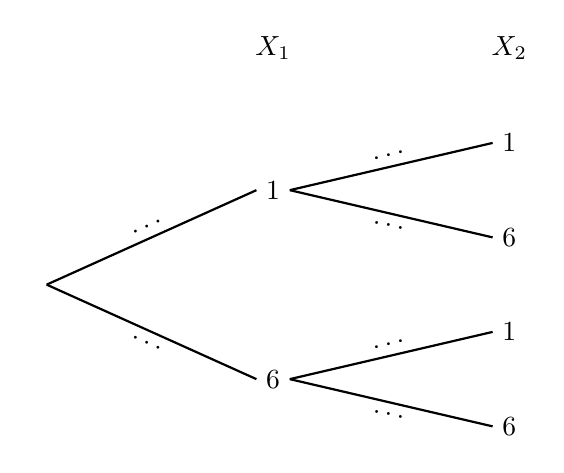
\begin{tikzpicture}[xscale=1,yscale=1]
		% Styles (MODIFIABLES)
		\tikzstyle{fleche}=[-,>=latex,thick]
		\tikzstyle{noeud}=[rounded corners=5pt]
		\tikzstyle{feuille}=[]
		\tikzstyle{commentaire}=[black]
		% Dimensions (MODIFIABLES)
		\def\DistanceInterNiveaux{3}
		\def\DistanceInterFeuilles{1.2}
		% Dimensions calculées (NON MODIFIABLES)
		\def\NiveauA{(0)*\DistanceInterNiveaux}
		\def\NiveauB{(1.0)*\DistanceInterNiveaux}
		\def\NiveauC{(2.0)*\DistanceInterNiveaux}
		\def\NiveauD{(3.000)*\DistanceInterNiveaux}
		\def\NiveauE{(4.5)*\DistanceInterNiveaux}
		\def\InterFeuilles{(-1)*\DistanceInterFeuilles}
		% Noeuds (MODIFIABLES : Styles et Coefficients d'InterFeuilles)
		\node[commentaire] (epreuve1) at ({\NiveauB},{(-1)*\InterFeuilles}) {$X_1$};
		\node[commentaire] (epreuve2) at ({\NiveauC},{(-1)*\InterFeuilles}) {$X_2$}; 
		%	\node[commentaire] (issues) at ({\NiveauD},{(-1)*\InterFeuilles}) {Issues};
		%	\node[commentaire] (probas) at ({\NiveauE},{(-1)*\InterFeuilles}) {Probabilités totales $Y=X_1+X_2$};
		% 
		\node[noeud] (R) at ({\NiveauA},{(1.5)*\InterFeuilles}) {};
		\node[noeud] (Ra) at ({\NiveauB},{(0.5)*\InterFeuilles}) {$1$};
		\node[feuille] (Raa) at ({\NiveauC},{(0)*\InterFeuilles}) {$1$}; 
		\node[feuille] (Rab) at ({\NiveauC},{(1)*\InterFeuilles}) {$6$}; 
		\node[noeud] (Rb) at ({\NiveauB},{(2.5)*\InterFeuilles}) {$6$};
		\node[feuille] (Rba) at ({\NiveauC},{(2)*\InterFeuilles}) {$1$}; 
		\node[feuille] (Rbb) at ({\NiveauC},{(3)*\InterFeuilles}) {$6$}; 
		%
		%	\node[commentaire] (I1) at ({\NiveauD},{(0)*\InterFeuilles}) {$\{X_1=1\} \cap \{X_2=1\}$}; 
		%	\node[commentaire] (I2) at ({\NiveauD},{(1)*\InterFeuilles}) {$\{X_1=1\} \cap \{X_2=6\}$}; 
		%	\node[commentaire] (I3) at ({\NiveauD},{(2)*\InterFeuilles}) {$\{X_1=6\} \cap \{X_2=1\}$}; 
		%	\node[commentaire] (I4) at ({\NiveauD},{(3)*\InterFeuilles}) {$\{X_1=6\} \cap \{X_2=6\}$};
		%
		%	\node[commentaire] (P1) at ({\NiveauE},{(0)*\InterFeuilles}) { $P(Y=2)=$}; 
		%	\node[commentaire] (P2) at ({\NiveauE},{(1)*\InterFeuilles}){ }; 
		%	%	\draw (P2.east) node[anchor=west, commentaire] {Faux négatif};
		%	\node[commentaire] (P3) at ({\NiveauE},{(2)*\InterFeuilles}){ }; 
		%	%	\draw (P3.east) node[anchor=west, commentaire] {Faux positif};
		%	\node[commentaire] (P4) at ({\NiveauE},{(3)*\InterFeuilles}) {$P(Y=12)=$ }; 
		%	\draw[ ultra thick] ({\NiveauE-1},{(3.3)*\InterFeuilles}) -- ({\NiveauE+1},{(3.3)*\InterFeuilles}) ;
		%	\node[commentaire] (P5) at ({\NiveauE},{(3.5)*\InterFeuilles})  { $1 $}; 
		% Arcs (MODIFIABLES : Styles)
		\draw[fleche] (R.east)--(Ra.west) node[midway, above,sloped]{$\ldots$};
		\draw[fleche] (Ra.east)--(Raa.west) node[midway, above,sloped]{$\ldots$};
		\draw[fleche] (Ra.east)--(Rab.west) node[midway, below,sloped]{$\ldots$};
		\draw[fleche] (R.east)--(Rb.west) node[midway, below,sloped]{$\ldots$};
		\draw[fleche] (Rb.east)--(Rba.west) node[midway, above,sloped]{$\ldots$};
		\draw[fleche] (Rb.east)--(Rbb.west) node[midway, below,sloped]{$\ldots$};
	\end{tikzpicture}
}
\parbox{0.48\linewidth}{
	\begin{tabular}{|*2{c|}*6{c}|}
		\cline{3-8}
		\multicolumn{2}{c|}{\multirow{2}{*}{}} & \multicolumn{6}{c|}{Dé \no 2 : $X_2$}  \\ \cline{3-8}
		\multicolumn{2}{c|}{}   &   \rule{0em}{1.5em}$\qquad$ &   $\qquad$  & $\qquad$  &  $\qquad$ && \\ \hline
		\multirow{6}{*}{\rotatebox[origin=c]{90}{Dé \no 1 : $X_1$}}	
		&  $\qquad$  &  \rule{0em}{1.5em} &   &  &   && \\ %\cline{2-6}
		&  $\qquad$ & \rule{0pt}{1.5em}\rule{1.8em}{0em}  &  \rule{1.8em}{0em}  &  \rule{1.8em}{0em}&\rule{1.8em}{0em} &&\\ %\cline{2-6}
		&  $\qquad$ & \rule{0pt}{1.5em}\rule{1.8em}{0em}  &  \rule{1.8em}{0em}  &  \rule{1.8em}{0em}&\rule{1.8em}{0em} &&\\ %\cline{2-6}
		&  $\qquad$  & \rule{0pt}{1.5em}  &   &   & &&  \\ %\cline{2-6}
		&  $\qquad$  & \rule{0pt}{1.5em}  &   &   &  && \\ %\cline{2-6}
		& $\qquad$  &  \rule{0pt}{1.5em} &   &  &    && \\ \hline
	\end{tabular} 
}
\item Calculer  $\Expect{Y}$. Que constatez vous ?
\end{enumerate}
\end{exercise}
\begin{exercise} On lance au plus trois fois une pièce bien équilibrée, et on s'arrète dès que l'on a obtenu \og Pile \fg. Les issues de cette expérience peuvent s'écrire : $P$,~ $FP$,~$FFP$ et $FFF$. \\
	La variable aléatoire $X$ correspond au  nombre total de lancers.
	\begin{enumerate}[leftmargin=*,label=\arabic*)]
	\item Les issues sont-elles équiprobables ?
	\item En complétant l'arbre de probabilité déterminer les probabilités des issues.\\
	\null\hfill 
	\begin{tikzpicture}[xscale=1,yscale=1]
		% Styles (MODIFIABLES)
		\tikzstyle{fleche}=[-,>=latex,thick]
		\tikzstyle{noeud}=[rounded corners=5pt]
		\tikzstyle{feuille}=[]
		\tikzstyle{commentaire}=[black]
		% Dimensions (MODIFIABLES)
		\def\DistanceInterNiveaux{3}
		\def\DistanceInterFeuilles{1.1}
		% Dimensions calculées (NON MODIFIABLES)
		\def\NiveauA{(0)*\DistanceInterNiveaux}
		\def\NiveauB{(0.750)*\DistanceInterNiveaux}
		\def\NiveauC{(1.5)*\DistanceInterNiveaux}
		\def\NiveauD{(2.250)*\DistanceInterNiveaux}
		\def\NiveauE{(3.0)*\DistanceInterNiveaux}
		\def\NiveauF{(3.75)*\DistanceInterNiveaux}
		\def\NiveauG{(4.5)*\DistanceInterNiveaux}
		\def\InterFeuilles{(-1)*\DistanceInterFeuilles}
		% Noeuds (MODIFIABLES : Styles et Coefficients d'InterFeuilles)
		\node[commentaire] (epreuve1) at ({\NiveauB},{(0.5)*\InterFeuilles}) {\scriptsize lancer \no 1};
		\node[commentaire] (epreuve2) at ({\NiveauC},{(0.5)*\InterFeuilles}) {\scriptsize lancer \no 2}; 
		\node[commentaire] (epreuve3) at ({\NiveauD},{(0.5)*\InterFeuilles}) {\scriptsize lancer \no 3};
		\node[commentaire] (issues) at ({\NiveauE},{(0.5)*\InterFeuilles}) {\scriptsize issues};
		\node[commentaire] (va) at ({\NiveauF},{(0.5)*\InterFeuilles}) {\scriptsize  valeurs de $X$};
		% 
		\node[noeud] (R) at ({\NiveauA},{(2)*\InterFeuilles}) {};
		\node[noeud] (Ra) at ({\NiveauB},{(1)*\InterFeuilles}) {P};
%		\node[feuille] (Raa) at ({\NiveauC},{(0.5)*\InterFeuilles}) {2};  
%		\node[feuille] (Raaa) at ({\NiveauD},{(0.5)*\InterFeuilles}) {3}; 
%		\node[feuille] (Rab) at ({\NiveauC},{(2)*\InterFeuilles}) { }; 
		\node[noeud] (Rb) at ({\NiveauB},{(3.0)*\InterFeuilles}) {F};
		\node[feuille] (Rba) at ({\NiveauC},{(2)*\InterFeuilles}) { }; 
		\node[noeud] (Rbb) at ({\NiveauC},{(4)*\InterFeuilles}) { }; 
			\node[feuille] (Rbba) at ({\NiveauD},{(3)*\InterFeuilles}) { }; 
			\node[feuille] (Rbbb) at ({\NiveauD},{(5)*\InterFeuilles}) { }; 
%		\node[noeud] (Rc) at ({\NiveauB},{(5.5)*\InterFeuilles}) { };
%		\node[feuille] (Rca) at ({\NiveauC},{(5)*\InterFeuilles}) { }; 
%		\node[feuille] (Rcb) at ({\NiveauC},{(6)*\InterFeuilles}) { }; 
		%
		\node[commentaire] (I1) at ({\NiveauE},{(1)*\InterFeuilles}) { $P$ }; 
		\node[commentaire] (I2) at ({\NiveauE},{(2)*\InterFeuilles}) {$\ldots$}; 
		%	\node[commentaire] (I3) at ({\NiveauD},{(2.25)*\InterFeuilles}) {$\overline{A}\cap B$}; 
		%	\node[commentaire] (I4) at ({\NiveauD},{(3.25)*\InterFeuilles}) {$\overline{A}\cap \overline{B}$};
		%	%
		\node[commentaire] (P1) at ({\NiveauF},{(1)*\InterFeuilles}) {$X=1$};  
		\node[commentaire] (Q1) at ({\NiveauG},{(1)*\InterFeuilles}) {$p_1=$}; 
		\node[commentaire] (P2) at ({\NiveauF},{(2)*\InterFeuilles}) {$X=\ldots$};
		%	%	\draw (P2.east) node[anchor=west, commentaire] {Faux négatif};
		%	\node[commentaire] (P3) at ({\NiveauE},{(2.25)*\InterFeuilles}){$P(\overline{A}\cap B)= $}; 
		%	%	\draw (P3.east) node[anchor=west, commentaire] {Faux positif};
		%	\node[commentaire] (P4) at ({\NiveauE},{(3.25)*\InterFeuilles}) {$P(\overline{A}\cap \overline{B})=$}; 
		%	%		\draw[ ultra thick] ({\NiveauE-1},{(3.55)*\InterFeuilles}) -- ({\NiveauE+1},{(3.55)*\InterFeuilles}) ;
		%	%		\node[commentaire] (P5) at ({\NiveauE},{(3.75)*\InterFeuilles})  {\textbf{Total}$=\ldots $}; 
		%	
		% Arcs (MODIFIABLES : Styles)
		\draw[fleche] (R.east)--(Ra.west) node[midway, above,sloped]{$\ldots$};
%		\draw[fleche] (Ra.east)--(Raa.west) node[midway, above]{ };
%		\draw[fleche] (Raa.east)--(Raaa.west) node[midway, above]{ };
		%		\draw[fleche] (Ra.east)--(Rab.west) node[midway, below]{};
		\draw[fleche] (R.east)--(Rb.west) node[midway, above,sloped]{$\ldots$};
			\draw[fleche] (Rb.east)--(Rba.west) node[midway, above,sloped]{$\ldots$};
			\draw[fleche] (Rb.east)--(Rbb.west) node[midway, below,sloped]{$\ldots$}; 
				\draw[fleche] (Rbb.east)--(Rbba.west) node[midway, below,sloped]{$\ldots$};
				\draw[fleche] (Rbb.east)--(Rbbb.west) node[midway, below,sloped]{$\ldots$};
%		\draw[fleche] (R.east)--(Rc.west) node[midway, below]{};
		%		\draw[fleche] (Rc.east)--(Rca.west) node[midway, above]{};
		%		\draw[fleche] (Rc.east)--(Rcb.west) node[midway, below]{};
	\end{tikzpicture} 
	\hfill \null  
	\item Déterminer la loi de probabilité de $X$ et la résumer dans un tableau.
	\item  En déduire $\Expect{X}$ et interpréter le résultat.
\end{enumerate} 
\end{exercise} 
\begin{exercise} On lance au plus quatre fois un dé équilibré d6, et on s'arrète dès que l'on a obtenu un $6$. La variable aléatoire $X$ correspond au nombre total de lancers réalisés. À l'aide d'un arbre identifier  la loi de probabilité de $X$ et déterminer $\Expect{X}$.
\end{exercise} 


\begin{exercise}[Point calculatrice]
	Pour chacune des variables aléatoires suivantes dont on donne la loi de probabilité à l'aide d'un tableau. Déterminer l'espérance, la variance et l'écart-type \textbf{	en rappellant les formules du cours} (on arrondira les résultats à $0,01$ près).
	
	\medskip
	\noindent\renewcommand{\arraystretch}{1.5}
	\ \begin{tabular}{|c|c|c|c|c|}
		\hline
		\cellcolor{blue!10}{$x_i$} & $-4$ & $0$ & $9$ & $25$ \\\hline
		\cellcolor{blue!10}{\scriptsize$P(X=x_i)$} & $0,5$ & $0,2$ & $0,2$ & $0,1$\\\hline
	\end{tabular} 
		\renewcommand{\arraystretch}{1.5}
		 \begin{tabular}{|c|c|c|c|c|}
			\hline
			\cellcolor{blue!10}{$x_i$} & $-25$ & $-3$ & $5$ & $100$ \\\hline
			\cellcolor{blue!10}{\scriptsize$P(Y=x_i)$} & $\frac{1}{3}$ & $\frac{1}{6}$ & $0,3$ & $0,2$\\\hline
		\end{tabular}  
		\renewcommand{\arraystretch}{1.5}
		 \begin{tabular}{|c|c|c|c|c|}
			\hline 	
				\cellcolor{blue!10}{$x_i$} & $-5$ & $0$ & $4$ & $10$ \\\hline
			\cellcolor{blue!10}{\scriptsize$P(Z=x_i)$} & $0,42$ & $0,38$ & $0,15$ & $0,05$\\\hline
		\end{tabular} 
	\smallskip
\end{exercise}

\begin{exercise}
	Une urne contient 3 boules bleues et deux boules rouges indiscernables au toucher. On tire successivement et sans remise 3 boules. 
	$X$ designe le nombre de boules bleues tirées.
	
	\begin{enumerate}[leftmargin=*,label=\arabic*)] 
		\item Compléter l'arbre de probabilité ci-dessous et identifier les valeurs possibles de $X$.\\
		\null\hfill 
		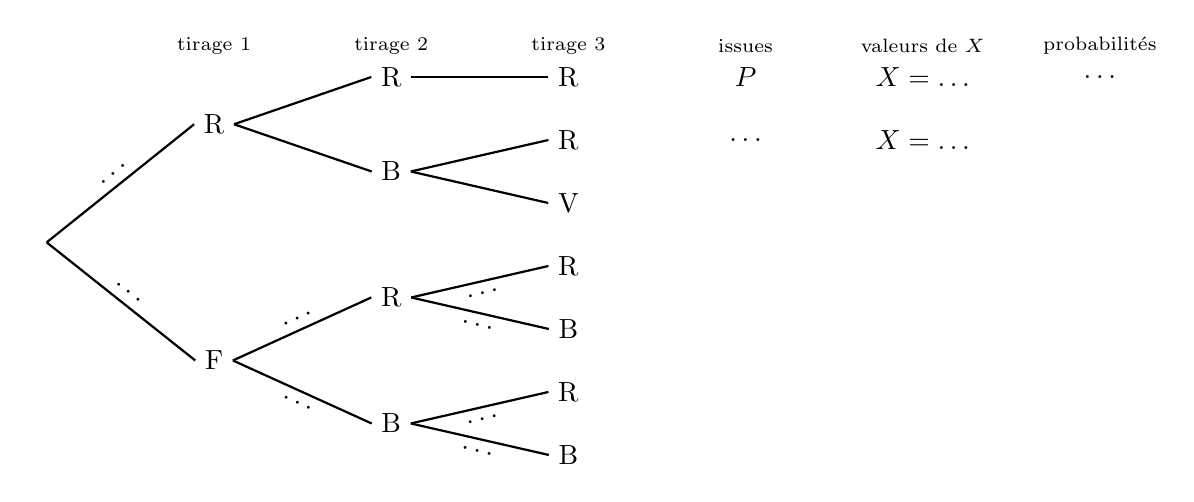
\begin{tikzpicture}[xscale=1,yscale=1]
			% Styles (MODIFIABLES)
			\tikzstyle{fleche}=[-,>=latex,thick]
			\tikzstyle{noeud}=[rounded corners=5pt]
			\tikzstyle{feuille}=[]
			\tikzstyle{commentaire}=[black]
			% Dimensions (MODIFIABLES)
			\def\DistanceInterNiveaux{3}
			\def\DistanceInterFeuilles{0.8}
			% Dimensions calculées (NON MODIFIABLES)
			\def\NiveauA{(0)*\DistanceInterNiveaux}
			\def\NiveauB{(0.750)*\DistanceInterNiveaux}
			\def\NiveauC{(1.5)*\DistanceInterNiveaux}
			\def\NiveauD{(2.250)*\DistanceInterNiveaux}
			\def\NiveauE{(3.0)*\DistanceInterNiveaux}
			\def\NiveauF{(3.75)*\DistanceInterNiveaux}
			\def\NiveauG{(4.5)*\DistanceInterNiveaux}
			\def\InterFeuilles{(-1)*\DistanceInterFeuilles}
			% Noeuds (MODIFIABLES : Styles et Coefficients d'InterFeuilles)
			\node[commentaire] (epreuve1) at ({\NiveauB},{(0.5)*\InterFeuilles}) {\scriptsize tirage \no 1};
			\node[commentaire] (epreuve2) at ({\NiveauC},{(0.5)*\InterFeuilles}) {\scriptsize tirage \no 2}; 
			\node[commentaire] (epreuve3) at ({\NiveauD},{(0.5)*\InterFeuilles}) {\scriptsize tirage \no 3};
			\node[commentaire] (issues) at ({\NiveauE},{(0.5)*\InterFeuilles}) {\scriptsize issues};
			\node[commentaire] (va) at ({\NiveauF},{(0.5)*\InterFeuilles}) {\scriptsize  valeurs de $X$};
			\node[commentaire] (va) at ({\NiveauG},{(0.5)*\InterFeuilles}) {\scriptsize  probabilités};
			% 
			\node[noeud] (R) at ({\NiveauA},{(3.625)*\InterFeuilles}) {};
			\node[noeud] (Ra) at ({\NiveauB},{(1.75)*\InterFeuilles}) {R};
			\node[feuille] (Raa) at ({\NiveauC},{(1)*\InterFeuilles}) {R};  
			\node[feuille] (Raaa) at ({\NiveauD},{(1)*\InterFeuilles}) {R}; 
			\node[feuille] (Rab) at ({\NiveauC},{(2.5)*\InterFeuilles}) {B}; 
			\node[feuille] (Raba) at ({\NiveauD},{(2)*\InterFeuilles}) {R}; 
			\node[feuille] (Rabb) at ({\NiveauD},{(3)*\InterFeuilles}) {V}; 
			\node[noeud] (Rb) at ({\NiveauB},{(5.5)*\InterFeuilles}) {F};
			\node[noeud] (Rba) at ({\NiveauC},{(4.5)*\InterFeuilles}) {R}; 
			\node[feuille] (Rbaa) at ({\NiveauD},{(4)*\InterFeuilles}) {R}; 
			\node[feuille] (Rbab) at ({\NiveauD},{(5)*\InterFeuilles}) {B}; 
			\node[noeud] (Rbb) at ({\NiveauC},{(6.5)*\InterFeuilles}) {B}; 
			\node[feuille] (Rbba) at ({\NiveauD},{(6)*\InterFeuilles}) {R}; 
			\node[feuille] (Rbbb) at ({\NiveauD},{(7)*\InterFeuilles}) {B}; 
			%			%		\node[noeud] (Rc) at ({\NiveauB},{(5.5)*\InterFeuilles}) { };
			%		\node[feuille] (Rca) at ({\NiveauC},{(5)*\InterFeuilles}) { }; 
			%		\node[feuille] (Rcb) at ({\NiveauC},{(6)*\InterFeuilles}) { }; 
			%
			\node[commentaire] (I1) at ({\NiveauE},{(1)*\InterFeuilles}) { $P$ }; 
			\node[commentaire] (I2) at ({\NiveauE},{(2)*\InterFeuilles}) {$\ldots$}; 
			%	\node[commentaire] (I3) at ({\NiveauD},{(2.25)*\InterFeuilles}) {$\overline{A}\cap B$}; 
			%	\node[commentaire] (I4) at ({\NiveauD},{(3.25)*\InterFeuilles}) {$\overline{A}\cap \overline{B}$};
			%	%
			\node[commentaire] (P1) at ({\NiveauF},{(1)*\InterFeuilles}) {$X=\ldots$};  
			\node[commentaire] (Q1) at ({\NiveauG},{(1)*\InterFeuilles}) {$\ldots$}; 
			\node[commentaire] (P2) at ({\NiveauF},{(2)*\InterFeuilles}) {$X=\ldots$};
			%	%	\draw (P2.east) node[anchor=west, commentaire] {Faux négatif};
			%	\node[commentaire] (P3) at ({\NiveauE},{(2.25)*\InterFeuilles}){$P(\overline{A}\cap B)= $}; 
			%	%	\draw (P3.east) node[anchor=west, commentaire] {Faux positif};
			%	\node[commentaire] (P4) at ({\NiveauE},{(3.25)*\InterFeuilles}) {$P(\overline{A}\cap \overline{B})=$}; 
			%	%		\draw[ ultra thick] ({\NiveauE-1},{(3.55)*\InterFeuilles}) -- ({\NiveauE+1},{(3.55)*\InterFeuilles}) ;
			%	%		\node[commentaire] (P5) at ({\NiveauE},{(3.75)*\InterFeuilles})  {\textbf{Total}$=\ldots $}; 
			%	
			% Arcs (MODIFIABLES : Styles)
			\draw[fleche] (R.east)--(Ra.west) node[midway, above,sloped]{$\ldots$};
			\draw[fleche] (Ra.east)--(Raa.west) node[midway, above]{ };
			\draw[fleche] (Raa.east)--(Raaa.west) node[midway, above]{ };
			\draw[fleche] (Ra.east)--(Rab.west) node[midway, below]{};
			\draw[fleche] (Rab.east)--(Raba.west) node[midway, above]{ };
			\draw[fleche] (Rab.east)--(Rabb.west) node[midway, above]{ };
			\draw[fleche] (R.east)--(Rb.west) node[midway, above,sloped]{$\ldots$};
			\draw[fleche] (Rb.east)--(Rba.west) node[midway, above,sloped]{$\ldots$};
			\draw[fleche] (Rba.east)--(Rbaa.west) node[midway, below,sloped]{$\ldots$};
			\draw[fleche] (Rba.east)--(Rbab.west) node[midway, below,sloped]{$\ldots$};
			\draw[fleche] (Rb.east)--(Rbb.west) node[midway, below,sloped]{$\ldots$}; 
			\draw[fleche] (Rbb.east)--(Rbba.west) node[midway, below,sloped]{$\ldots$};
			\draw[fleche] (Rbb.east)--(Rbbb.west) node[midway, below,sloped]{$\ldots$};
			%		\draw[fleche] (R.east)--(Rc.west) node[midway, below]{};
			%		\draw[fleche] (Rc.east)--(Rca.west) node[midway, above]{};
			%		\draw[fleche] (Rc.east)--(Rcb.west) node[midway, below]{};
		\end{tikzpicture} 
		\hfill \null   
		\item Déterminer la loi de probabilité de $X$\\
		\renewcommand{\arraystretch}{1.1} 
		\null	\hfill \begin{tabularx}{0.7\linewidth}{|c|Y|Y|Y|c|}
			\hline
			\cellcolor{blue!10}{$x$} & $1$ & $2$ & $3$ & \textbf{Total}\\ \hline
			\cellcolor{blue!10}{$P(X=x)$} &   &    &   & \\\hline
			%			\cellcolor{blue!10}{$P(X=x)$} & $\tfrac{3}{10}$ & $\tfrac{6}{10}$  & $\tfrac{1}{10}$  & \\\hline
		\end{tabularx} 
		\hfill \null
		\item En déduire l'espérance  $\Expect{X}$, la variance $\Var{X}$ et l'écart type $\sigma(X)$.
	\end{enumerate} 
\end{exercise}
\begin{exercise}[Examen blanc type E3C]\hfill \\%sujet 45 exercice 2
	Une urne contient deux boules rouges et trois boules noires toutes indiscernables au toucher.  On tire au hasard une première boule en notant sa couleur puis on la remet dans l'urne.  
	On tire ensuite toujours au hasard une deuxième boule en notant sa couleur.  
\begin{enumerate}[label=\arabic*),leftmargin=*]
	\item 	On note $R$ l'évènement \og tirer une boule rouge \fg{} et $N$ l'évènement \og tirer une boule noire \fg. Compléter   l'arbre de probabilité ci-dessous associé à cette expérience. \\
\noindent \parbox{1\linewidth}{\centering
	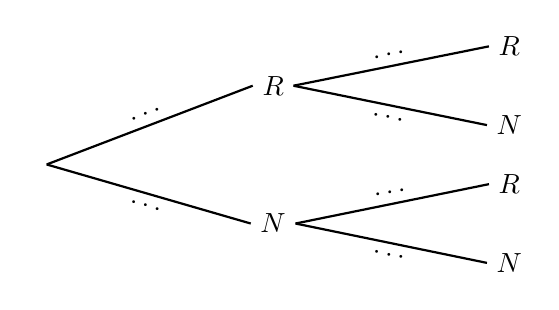
\begin{tikzpicture}[xscale=1,yscale=1]
		% Styles (MODIFIABLES)
		\tikzstyle{fleche}=[-,>=latex,thick]
		\tikzstyle{noeud}=[rounded corners=5pt]
		\tikzstyle{feuille}=[]
		\tikzstyle{commentaire}=[black]
		% Dimensions (MODIFIABLES)
		\def\DistanceInterNiveaux{3}
		\def\DistanceInterFeuilles{1.0}
		% Dimensions calculées (NON MODIFIABLES)
		\def\NiveauA{(0)*\DistanceInterNiveaux}
		\def\NiveauB{(1.0)*\DistanceInterNiveaux}
		\def\NiveauC{(2.0)*\DistanceInterNiveaux}
		\def\NiveauD{(2.750)*\DistanceInterNiveaux}
		\def\NiveauE{(3.5)*\DistanceInterNiveaux}
		\def\InterFeuilles{(-1)*\DistanceInterFeuilles}
		% Noeuds (MODIFIABLES : Styles et Coefficients d'InterFeuilles)
		%	\node[commentaire] (epreuve1) at ({\NiveauB},{(0)*\InterFeuilles}) {\scriptsize Observation};
		%	\node[commentaire] (epreuve2) at ({\NiveauC},{(0)*\InterFeuilles}) {\scriptsize Cause}; 
		%	\node[commentaire] (issues) at ({\NiveauD},{(0)*\InterFeuilles}) {\scriptsize Issues};
		%	\node[commentaire] (probas) at ({\NiveauE},{(0)*\InterFeuilles}) {\scriptsize Probabilités};
		% 
		\node[noeud] (R) at ({\NiveauA},{(2.00)*\InterFeuilles}) {};
		\node[noeud] (Ra) at ({\NiveauB},{(1)*\InterFeuilles}) {$R$};
		\node[feuille] (Raa) at ({\NiveauC},{(0.5)*\InterFeuilles}) {$R$}; 
		\node[feuille] (Rab) at ({\NiveauC},{(1.5)*\InterFeuilles}) {${N}$}; 
		\node[noeud] (Rb) at ({\NiveauB},{(2.75)*\InterFeuilles}) {$N$};
		\node[feuille] (Rba) at ({\NiveauC},{(2.25)*\InterFeuilles}) {$R$}; 
		\node[feuille] (Rbb) at ({\NiveauC},{(3.25)*\InterFeuilles}) {${N}$}; 
		%
		%	\node[commentaire] (I1) at ({\NiveauD},{(0.5)*\InterFeuilles}) {$A\cap B$}; 
		%	\node[commentaire] (I2) at ({\NiveauD},{(1.5)*\InterFeuilles}) {$A\cap \overline{B}$}; 
		%	\node[commentaire] (I3) at ({\NiveauD},{(2.25)*\InterFeuilles}) {$\overline{A}\cap B$}; 
		%	\node[commentaire] (I4) at ({\NiveauD},{(3.25)*\InterFeuilles}) {$\overline{A}\cap \overline{B}$};
		%	%
		%	\node[commentaire] (P1) at ({\NiveauE},{(0.5)*\InterFeuilles}) {$P(A\cap B)= $}; 
		%	\node[commentaire] (P2) at ({\NiveauE},{(1.5)*\InterFeuilles}){$P(A\cap \overline{B})= $}; 
		%	%	\draw (P2.east) node[anchor=west, commentaire] {Faux négatif};
		%	\node[commentaire] (P3) at ({\NiveauE},{(2.25)*\InterFeuilles}){$P(\overline{A}\cap B)= $}; 
		%	%	\draw (P3.east) node[anchor=west, commentaire] {Faux positif};
		%	\node[commentaire] (P4) at ({\NiveauE},{(3.25)*\InterFeuilles}) {$P(\overline{A}\cap \overline{B})=$}; 
		%	%		\draw[ ultra thick] ({\NiveauE-1},{(3.55)*\InterFeuilles}) -- ({\NiveauE+1},{(3.55)*\InterFeuilles}) ;
		%	%		\node[commentaire] (P5) at ({\NiveauE},{(3.75)*\InterFeuilles})  {\textbf{Total}$=\ldots $}; 
		%	
		% Arcs (MODIFIABLES : Styles)
		\draw[fleche] (R.east)--(Ra.west) node[midway, sloped, above]{$\ldots$};
		\draw[fleche] (Ra.east)--(Raa.west) node[midway, sloped, above]{$\ldots$};
		\draw[fleche] (Ra.east)--(Rab.west) node[midway, sloped, below]{$\ldots$};
		\draw[fleche] (R.east)--(Rb.west) node[midway, sloped, below]{$\ldots$};
		\draw[fleche] (Rb.east)--(Rba.west) node[midway, sloped, above]{$\ldots$};
		\draw[fleche] (Rb.east)--(Rbb.west) node[midway, sloped, below]{$\ldots$};
	\end{tikzpicture} 
} 
	\item Quelle est la probabilité de tirer deux boules rouges ?
	\item Si un joueur tire une boule rouge, il gagne $20$ euros. S'il tire une boule noire, il perd $10$ euros. 
	
	On note $X$ la variable aléatoire égale au gain algébrique du joueur, en euros, à l'issue des deux tirages successifs. 
	Déterminer la loi de probabilité de la variable aléatoire $X$.
	\item Calculer la probabilité que le joueur gagne de l'argent.
	\item Calculer l'espérance de la variable aléatoire $X$ et en donner une interprétation.
	\end{enumerate}
	 
\end{exercise} 
%----------------------------------------------------------------------------------------
%	 
%---------------------------------------------------------------------------------------- 
\newpage 
\begin{exercise}[Formule de König-Huygens] Une V.A. réelle finie vérifie $\Var{X}=\Expect{X^2}-\big(\Expect{X}\big)^2$.   \\
	Complétez pour établir cette propriété dans le cas simplifié ou la V.A. $X$ ne prend que 4 valeurs : \\
	\renewcommand{\arraystretch}{1.25} 
	\null	\hfill \begin{tabularx}{0.7\linewidth}{|c|Y|Y|Y|Y|}
		\hline
		\cellcolor{blue!10}{$x$} & $x_1$ & $x_2$ & $x_3$ & $x_4$ \\ \hline
		\cellcolor{blue!10}{$P(X=x)$} & $p_1$ & $p_2$  & $p_3$  & $p_4$  \\\hline
	\end{tabularx} 
	\hfill \null
	\begin{spacing}{2}
		\begin{enumerate}[label={},leftmargin=*]  
			\item $\sum_{i=1}^{4}p_i=p_1+p_2+ p_3+p_4=$\dotfill
			\item $\mu=\Expect{X}=\sum_{i=1}^{4}x_ip_i=x_1p_1+\dotfill $
			\item $\Var{X}=\Expect{(X-\mu)^2} =\sum_{i=1}^4 (x_i   -\mu)^2p_i$
			\item $\Var{X}=\sum_{i=1}^4 (x_i^2-\ldots\ldots x_i + \ldots\ldots)p_i$
			\item $\Var{X}= (x_1^2-2\mu  x_1 + \mu^2)p_1+\dotfill $
			\item $\Var{X}=x_1^2p_1+ \dotfill -2\mu(x_1p_1+\dotfill )+ \mu^2(p_1+\dotfill)$
			\item $\Var{X}=\Expect{\ldots\ldots} \hfill -2\mu \Expect{\ldots\ldots} \hfill+ \mu^2\ldots\ldots$\hfill
			\item $\Var{X}=\Expect{\ldots\ldots} -2\mu \ldots\ldots + \mu^2\ldots\ldots$
			\item $\Var{X}=\Expect{\ldots\ldots} -  \ldots\ldots$
		\end{enumerate}
	\end{spacing} 
\end{exercise}
\vspace{-1.5em}
%\begin{remark} Comme la variance est positive, on déduit que $\Expect{X^2}\geqslant (\Expect{X})^2$ 
%\end{remark}
\begin{exercise}Utiliser la formule de König-Huygens pour déterminer les variances des v.a. $X$ et $Y$ dont les loies sont décrites dans le tableau ci-dessous :\\
	\renewcommand{\arraystretch}{1.25} 
	\null	\hfill \begin{tabularx}{0.7\linewidth}{|c|Y|Y|Y|Y|Y|}
		\hline
		\cellcolor{blue!10}{$x_i$} & $1$ & $2$ & $3$ & $4$ & $5$ \\ \hline
		\cellcolor{blue!10}{$P(X=x_i)$} & $0.2$ & $0.2$  & $0.2$  & $0.2$   & $0.2$  \\\hline
		\cellcolor{blue!10}{$P(Y=x_i)$} & $0.02$ & $0.18$  & $0.61$  & $0.16$   & $0.03$  \\\hline
	\end{tabularx} 
	\hfill \null 
\end{exercise}
\begin{exercise} On considère la v.a. qui prend les valeurs $0$ et $1$, avec $P(X=1)=p$.
	\begin{enumerate}[label={\arabic*)},leftmargin=*]  
		\item Exprimer $q=P(X=0)$ en fonction de $p$
		\item Montrer que $\Expect{X}=p$ et   $\Var{X}=pq$. 
	\end{enumerate}
\end{exercise}
\begin{exercise} On lance un dé équilibré. On note $X$ la v.a. correspondant au nombre obtenu. Complétez pour déterminer ses paramètres $\mu$ et $\sigma$ :
	\vspace{-0.5em}
	\begin{spacing}{1.8}
		\begin{enumerate}[label={},leftmargin=*]  
			\item  $\mu=\Expect{X}=1\times \ldots\ldots+2\times \ldots\ldots+3\times \ldots\ldots+4\times \ldots\ldots+5\times \ldots\ldots+6\times \ldots\ldots$
			\item $\mu=\frac{1+2+3+4+5+6}{\qquad}=\dotfill $
			\item $\Expect{X^2}=1^2\times \ldots\ldots+2^2\times \ldots\ldots+3^2\times \ldots\ldots+4^2\times \ldots\ldots+5^2\times \ldots\ldots+6^2\times \ldots\ldots$
			\item $\Expect{X^2}=\frac{1^2+2^2+3^2+4^2+5^2+6^2}{\qquad}=\dotfill $
			\item $\Var{X}=\Expect{X^2}-\ldots\ldots\ldots = \dotfill$
			\item $\sigma=$\dotfill
		\end{enumerate}
	\end{spacing} 
\end{exercise} 
\vspace{-1em} 
\begin{exercise} Soit une variable aléatoire finie $X$, et $a$ et $b\in\mathbb{R}$. Alors on a :
	\setlength{\abovedisplayskip}{3pt}
	\setlength{\belowdisplayskip}{3pt}  
	\begin{align*}
		\Expect{aX}&=a\Expect{X}\\
		\Expect{X+b}&=\Expect{X}+b \\
		\text{formules que l'on regroupe dans}\qquad \Expect{aX+b}&=a\Expect{X}+b
	\end{align*}
	%	$$\Expect{aX+b}=a\Expect{X}+b$$ 
	%$$\Var{aX+b}=a^ 2\Var{X}$$ 
	Complétez pour établir cette propriété dans le cas simplifié ou la V.A. $X$ ne prend que 4 valeurs :\\
	\renewcommand{\arraystretch}{1.25} 
	\null	\hfill \begin{tabularx}{0.7\linewidth}{|c|Y|Y|Y|Y|}
		\hline
		\cellcolor{blue!10}{$x$} & $x_1$ & $x_2$ & $x_3$ & $x_4$ \\ \hline
		\cellcolor{blue!10}{$P(X=x)$} & $p_1$ & $p_2$  & $p_3$  & $p_4$  \\\hline
	\end{tabularx} 
	\hfill \null
	\begin{spacing}{2}
		\begin{enumerate}[label={},leftmargin=*]
			\item $\sum_{i=1}^{4}p_i=p_1+p_2+ p_3+p_4=$\dotfill
			\item $\Expect{X}=\sum_{i=1}^{4}x_ip_i=x_1p_1+\dotfill $
			\item $\Expect{aX+b}=\sum_{i=1}^{4}(ax_i+b)p_i=(ax_1+b)p_1+\dotfill $
			\item  $\Expect{aX+b}=ax_1p_1 + bp_1+\dotfill $
			\item $\Expect{aX+b}=ax_1p_1 + \dotfill + bp_1+\dotfill $
			\item $\Expect{aX+b}=a(x_1p_1+x_2p_2+\dotfill) + b(p_1+p_2+\dotfill) $
			\item $\Expect{aX+b}=a\ldots\ldots\ldots+ b \ldots\ldots $ 
		\end{enumerate}
%			\begin{enumerate}[label={},leftmargin=*]
%					\item $\Var{aX+b}=\Expect{(aX+b- \Expect{aX+b})^2}$
%					\item $\Var{aX+b}=\Expect{(aX+b- (a\Expect{X}+b))^2}$
%					\item $\Var{aX+b}=\Expect{(aX+b- a\Expect{X}\ldots b)^2}$
%					\item $\Var{aX+b}=\Expect{(aX+b- a\Expect{X}\ldots b)^2}$
%					\item $\Var{aX+b}=\Expect{(aX- a\Expect{X})^2}$
%					\item $\Var{aX+b}=\Expect{\ldots (X- \Expect{X})^2}$
%					\item $\Var{aX+b}=\ldots\ldots\Expect{ (X- \Expect{X})^2}$ 
%					\end{enumerate}
	\end{spacing}
\end{exercise}
%\begin{remark} Pour une V.A. finie $\Expect{X^r}$ est le moment d'ordre $r\in\mathbb{N}$ :
%\begin{enumerate}[label={},leftmargin=*]
%	\item $\Expect{X^1}=\Expect{X}=\sum_{i=1}^n x_iP(X=x_i)$ est le moment d'ordre 1.
%	\item $\Expect{X^2}=\Expect{X^2}=\sum_{i=1}^n x_i^2P(X=x_i)$  est le moment d'ordre 2.
%\end{enumerate} 
%\end{remark}
\vspace{-1.5em} 
\begin{exercise} Une entreprise compte 100 salariés. Le tableau de répartitions des salaires est  :\\
	\renewcommand{\arraystretch}{1.25} 
	\null	\hfill \begin{tabularx}{0.7\linewidth}{|c|Y|Y|Y|Y|}
		\hline
		\cellcolor{blue!10}{Salaire en \euro} & $1550$ & $1750$ & $2200$ & $3000$ \\ \hline
		\cellcolor{blue!10}{Nb de personnes} & $40$ & $35$  & $24$  & $1$  \\\hline
	\end{tabularx} 
	\hfill \null\\
	On tire un employé au hasard. On note $X$ la v.a. correspondant au salaire perçu.
	\begin{enumerate}[label={\arabic*)},leftmargin=*]  
		\item Déterminer $\Expect{X}$.
		\item Le directeur décide d'augmenter tous les salaires de \EUR{10}. Que devient l'espérance ?
		\item Le directeur décide d'augmenter les salaires de 2\%. Comment évolue l'espérance ?
	\end{enumerate}
\end{exercise}
\begin{exercise}  $X$ est une v.a. prenant 4 valeurs. \\
Soit la fonction $f$ définie sur $\mathbb{R}$ par $f(x)=\Expect{(X-x)^2}$
	\begin{enumerate}[label={\arabic*)},leftmargin=*]  
		\item Montrer que $f(x)=\sum_{i=1}^4(x_i-x)^2p_i=\Expect{X^2}-2x\Expect{X}+x^2$.
		\item Étudier les variations de $f$ sur $\mathbb{R}$.
		\item Montrer que $f$ admet un minimum et que ce minimum est atteint pour $x=\Expect{X}$.
	\end{enumerate}
\end{exercise}
 \begin{exercise} $X$ est une v.a. prenant 4 valeurs.  $a$ et $b\in\mathbb{R}$.
	\begin{enumerate}[label={\arabic*)},leftmargin=*]  
 		\item Montrer que $\Var{X+b}=\Var{X}$.
 		\item Montrer que $\Var{aX}=a^2X$
 		\item Exprimer $\sigma(aX+b)$ en fonction de $\sigma(X)$.
 	\end{enumerate}
 \end{exercise}
\begin{exercise} Soit une v.a. finie $X$. Expriquer pourquoi  $\Expect{X^2}\geqslant \big(\Expect{X}\big)^2$ 
\end{exercise} 
%----------------------------------------------------------------------------------------
%	 
%----------------------------------------------------------------------------------------

\newpage 
\begin{example}[Simuler une variable aléatoire de loi quelconque à partir d'une loi équiprobable]  \href{https://my.numworks.com/python/niz-moussatat/de_grim_magenta}{lien}\\
Soit le dé de Grim magenta  \begin{tikzpicture}[baseline]
	\tikzstyle{every cut}=[white]
		\tikzstyle{every fold}=[white]
		\path pic [
		folding line length=6.5mm,
		transform shape,
		rotate=90, 
		% numbered faces,
		face 1 = {\node {\Huge\epsdice[white]{1}};},
		face 2 = {\node {\Huge\epsdice[white]{1}};},
		face 3 = {\node {\Huge\epsdice[white]{6}};},
		face 4 = {\node {\Huge\epsdice[white]{6}};},
		face 5 = {\node {\Huge\epsdice[white]{6}};},
		face 6 = {\node {\Huge\epsdice[white]{6}};} 
		]
		{cube folding};
	\end{tikzpicture}.  

\noindent
%\parbox{0.48\linewidth}{
\begin{lstlisting}[ language=python , 
%	title=Script C,   
linewidth=1\columnwidth,
style=python-code,    
aboveskip=0.0\topskip,
belowskip=0.0\topskip,
xleftmargin=1.2em,
lineskip=0.3em,
tabsize=4, 
%numbers=none,
%	firstnumber=10  
caption={fonction \lstinline|magenta()| retourne une réalisation d'un lancer de dé magenta de Grim : $P(X=1)=\tfrac{2}{6}$ et $P(X=6)=\tfrac{4}{6}$}
] 
from random import randint 
def magenta() :	
	face = randint(1,6)
	if face <= 2 :
		return 1
	else :
		return 6 
\end{lstlisting} 



\noindent
\begin{minipage}{0.6\linewidth}
\noindent Pour simuler la variable aléatoire somme de deux dés de Grim magenta $S$ : $P(S=2)=\tfrac{4}{36}$ , $P(S=7)=\tfrac{16}{36}$ et $P(S=12)=\tfrac{16}{36}$ on peut procéder de deux manières :
	\begin{lstlisting}[ language=python , 
		%	title=Script C,   
		linewidth=1\columnwidth,
		style=python-code,    
		aboveskip=0.0\topskip,
		belowskip=0.0\topskip,
		xleftmargin=1.2em,
		lineskip=0.3em,
		tabsize=4, 
		%numbers=none,
		%	firstnumber=10  
		%caption={}
		]  
def double_magenta() :	
	total = magenta() + magenta() 
	return total
\end{lstlisting} 
\end{minipage}
\hfill
\begin{minipage}{0.38\linewidth}
\begin{lstlisting}[ language=python , 
%	title=Script C,   
linewidth=1\columnwidth,
style=python-code,    
aboveskip=0.0\topskip,
belowskip=0.0\topskip,
xleftmargin=1.2em,
lineskip=0.3em,
tabsize=4, 
%numbers=none,
%	firstnumber=10  
caption={fonction \lstinline|double_magenta()| retourne une réalisation de la variable aléatoire $S$.}
]  
def double_magenta() :	
	face = randint(1,36)
	if face <= 4 :
		return ....
	elif face <= .... :
		return 7
	else :
		return 12
\end{lstlisting} 
\end{minipage}


\noindent
\begin{minipage}{0.48\linewidth}
\begin{lstlisting}[ language=python , 
	%	title=Script C,   
	linewidth=1\columnwidth,
	style=python-code,    
	aboveskip=0.0\topskip,
	belowskip=0.0\topskip,
	xleftmargin=1.2em,
	lineskip=0.3em,
	tabsize=4, 
	%numbers=none,
	%	firstnumber=10  
	caption={fonction \lstinline|frequence_magenta(n)| retourne la fréquence relative de l'issue 1  pour \lstinline|n| répétitions du lancer d'un dé de Grim magenta.}
	]  
def frequence_magenta(n) :	
	compteur = 0
	for i in range(n) :
		lancer = magenta()
		if lancer == 1 :
			compteur = compteur + 1
	f = compteur/n
	return f
\end{lstlisting} 
\end{minipage}
\hfill
\begin{minipage}{0.48\linewidth}
\begin{lstlisting}[ language=python , 
%	title=Script C,   
linewidth=1\columnwidth,
style=python-code,    
aboveskip=0.0\topskip,
belowskip=0.0\topskip,
xleftmargin=1.2em,
lineskip=0.3em,
tabsize=4, 
%numbers=none,
%	firstnumber=10  
caption={fonction \lstinline|frequence_double_magenta(x,n)| retourne la fréquence relative de l'issue \lstinline|x|  pour \lstinline|n| répétitions d'un double lancer de dés magentas.}
]  
def frequence_double_magenta(x,n) :	
	compteur = 0
	for i in range(n) :
		lancer = ...
		if lancer == .... :
			compteur = compteur + 1
	f = compteur/n
	return f
\end{lstlisting} 
\end{minipage}


\noindent
\begin{minipage}{0.48\linewidth}
\begin{lstlisting}[ language=python , 
%	title=Script C,   
linewidth=1\columnwidth,
style=python-code,    
aboveskip=0.0\topskip,
belowskip=0.0\topskip,
xleftmargin=1.2em,
lineskip=0.3em,
tabsize=4, 
%numbers=none,
%	firstnumber=10  
caption={fonction \lstinline|moyenne_magenta(n)| retourne une estimation $\Expect{X}$ en calculant la valeur  moyenne \lstinline|n| répétitions.  }
]  
def moyenne_magenta(n) :	
	cumul = 0
	for i in range(n) :
		cumul = cumul + magenta()
	moyenne = cumul / n
	return moyenne
\end{lstlisting} 
\end{minipage}
\hfill
\begin{minipage}{0.48\linewidth}
	\begin{lstlisting}[ language=python , 
		%	title=Script C,   
		linewidth=1\columnwidth,
		style=python-code,    
		aboveskip=0.0\topskip,
		belowskip=0.0\topskip,
		xleftmargin=1.2em,
		lineskip=0.3em,
		tabsize=4, 
		%numbers=none,
		%	firstnumber=10  
		caption={fonction \lstinline|moyenne_double_magenta(n)| retourne une estimation $\Expect{S}$ en calculant la valeur  moyenne \lstinline|n| répétitions.   }
		]  
def moyenne_double_magenta(n) :	
	cumul = 0
	for i in range(n) :
		cumul = cumul + ...
	moyenne = cumul / n
	return moyenne
\end{lstlisting}  
\end{minipage} 
\end{example} 


\newpage 
\begin{exercise}[à vous \href{https://my.numworks.com/python/niz-moussatat/de_grim_vertvsjaune}{lien}]   
	Soit les dés de Grim jaune  (3~;~3~;~3~;~3~;~8~;~8)   
et vert (0~;~5~;~5~;~5~;~5~;~5). 
\begin{enumerate}[label=\arabic*),leftmargin=*]
	\item Écrire les fonctions \lstinline|jaune()| et \lstinline|rouge()| qui retournent l'issue d'un lancer de dé jaune et d'un rouge. \\
\noindent
\begin{minipage}{0.48\linewidth} 
\begin{lstlisting}[ language=python , 
	%	title=Script C,   
	linewidth=1\columnwidth,
	style=python-code,    
	aboveskip=0.0\topskip,
	belowskip=0.0\topskip,
	xleftmargin=1.2em,
	lineskip=0.3em,
	tabsize=4, 
	%numbers=none,
	%	firstnumber=10  
%	caption={}
	] 
from random import randint 
def jaune() :	
	face = randint(1,6)
	if face <= ... :
		return ...
	else :
		return ...
\end{lstlisting} 
\end{minipage}
\hfill 
\begin{minipage}{0.48\linewidth}
\begin{lstlisting}[ language=python , 
%	title=Script C,   
linewidth=1\columnwidth,
style=python-code,    
aboveskip=0.0\topskip,
belowskip=0.0\topskip,
xleftmargin=1.2em,
lineskip=0.3em,
tabsize=4, 
%numbers=none,
%	firstnumber=10  
%	caption={}
] 
from random import randint 
def vert() :	
	face = randint(1,6)
	if face <= ... :
		return ...
	else :
		return ...
\end{lstlisting} 
\end{minipage}
\item On fait jouer un dé vert contre un jaune. Déterminer $P(\text{Jaune}>\text{Vert})$ %4/9
\item On souhaite vérifier le résultat obtenu à la question précédente à l'aide d'un script Python. Complétez le script suivant afin que l'instruction \lstinline|frequence_jaunebatvert(n)| retourne la fréquence de victoire du dé jaune sur \lstinline|n| épreuves.

\begin{lstlisting}[ language=python , 
%	title=Script C,   
linewidth=1\columnwidth,
style=python-code,    
aboveskip=0.0\topskip,
belowskip=0.0\topskip,
xleftmargin=1.2em,
lineskip=0.3em,
tabsize=4, 
%numbers=none,
%	firstnumber=10  
%	caption={}
]  
def frequence_jaunebatvert(n) :	
	compteur = 0
	for i in .......... :
		j = ...
		v = ...
		if .......... :
			compteur = compteur + 1
	f = .....
	return f
\end{lstlisting} 
\item On affronte désormais une paire de dés jaunes avec une paire de dés vert en comparant le total de chaque paire. Dans le script ci-dessous l'instruction \lstinline|frequence_doublejaunebatdoublevert(n)| retourne la fréquence de victoire d'une paire de dés jaunes sur \lstinline|n| épreuves. Complétez et tester le script.
\begin{lstlisting}[ language=python , 
%	title=Script C,   
linewidth=1\columnwidth,
style=python-code,    
aboveskip=0.0\topskip,
belowskip=0.0\topskip,
xleftmargin=1.2em,
lineskip=0.3em,
tabsize=4, 
%numbers=none,
%	firstnumber=10  
%	caption={}
]  
def frequence_doublejaunebatdoublevert(n) :	
	compteur = 0
	for i in .......... :
		j = ...
		v = ...
		if .......... :
			compteur = compteur + 1		
	f = .....
	return f
\end{lstlisting} 
\item Que constatez vous ? Montrer que $P(\text{Double jaune}>\text{Double vert})=\tfrac{56}{81}$.
\item  	  Complétez le script pour calculer la valeur moyenne du total d'une paire de deux dés jaunes après \lstinline|n| répétitions. 
\begin{lstlisting}[ language=python , 
%	title=Script C,   
linewidth=1\columnwidth,
style=python-code,    
aboveskip=0.0\topskip,
belowskip=0.0\topskip,
xleftmargin=1.2em,
lineskip=0.5em,
tabsize=4, 
%numbers=none,
%	firstnumber=10  
%caption={ }
]  
def moyenne_double_jaune(n) :	
	cumul = ....
	for i in ........ :
		...
		...
	return ...
\end{lstlisting}  
\end{enumerate}
\end{exercise}  
%----------------------------------------------------------------------------------------
%	 
%---------------------------------------------------------------------------------------- 
\newpage 
\begin{eBox}
Dans Python, on peut créer et utiliser des listes (de lettres, de mots, de chiffres, ...).\\ 
\noindent Une liste est une suite d’éléments \textbf{numérotés} dont le \textbf{premier indice est 0} (on commence à compter à partir du rang 0).\\ Les éléments sont entre crochets \lstinline|[]| et séparés par des virgules.\\ 
Pour atteindre l’élément d’indice \og i \fg{} de la liste \og  \lstinline|L| \fg{}, il suffit d’écrire  \og  \lstinline|L[i]| \fg{}. 
\end{eBox}
\begin{example}\hfill \\
\noindent
\begin{minipage}{0.40\linewidth}
\begin{pyconsole}
L = ["P","I","Z","Z","A"]
L[1] 	# terme de rang 1
L[4]
L[0] 	# terme de rang 0
len(L)	# nbr d'éléments de L
L.append("S") 	
# ajoute élément en fin de L
L
M = [] 	# liste vide
len(M)
\end{pyconsole}
\end{minipage}
\hfill 
\begin{minipage}{0.55\linewidth}
\paragraph{Créer}    des listes \textbf{par compréhension} à l'aide de l'instruction \lstinline|for|  :
\begin{pyconsole}
ma_liste=[i**2+1 for i in range(5)] 
ma_liste 
\end{pyconsole}

ou à l'aide de la méthode  \lstinline|append| :
		
\begin{lstlisting}[ language=python , 
%	title=Script C,   
linewidth=1\columnwidth,
style=python-code,    
aboveskip=0.0\topskip,
belowskip=0.0\topskip,
xleftmargin=1.2em,
lineskip=0.5em,
tabsize=4, 
%numbers=none,
%	firstnumber=10  
%caption={ }
]  
ma_liste=[]		#liste vide
for i in range(5) :
	ma_liste.append(i**2+1)
\end{lstlisting} 

\paragraph{Parcourir}  une liste avec une boucle for :

\begin{lstlisting}[ language=python , 
%	title=Script C,   
linewidth=1\columnwidth,
style=python-code,    
aboveskip=0.0\topskip,
belowskip=0.0\topskip,
xleftmargin=1.2em,
lineskip=0.5em,
tabsize=4, 
%numbers=none,
%	firstnumber=10  
%caption={ }
]  
ma_liste = ['I','did','it','for','love']
for i in range(len(ma_liste)) :
	print(ma_liste[i])
\end{lstlisting} 
affiche :  
\begin{pycode}
ma_liste = ['I','did','it','for','love']
for i in range(5) :
	print(ma_liste[i])
\end{pycode}   
\end{minipage}
\end{example}
\begin{example}On reprend la fonction \lstinline|magenta()| qui simule le dé magenta de Grim. Ce script simule \lstinline|n| lancer de dés et calcule la moyenne des résultats de l'échantillon complet.\hfill 
\begin{lstlisting}[ language=python , 
	%	title=Script C,   
	linewidth=1\columnwidth,
	style=python-code,    
	aboveskip=0.0\topskip,
	belowskip=0.0\topskip,
	xleftmargin=1.2em,
	lineskip=0.5em,
	tabsize=4, 
	%numbers=none,
	%	firstnumber=10  
%caption={}
	]   
n=400       								# taille de l'échantillon		
echantillon=[magenta() for i in range(n)]	# liste des issues de n épreuves 
x = sum(echantillon)/n 						# moyenne de l'échantillon
\end{lstlisting} 
\begin{figure*}[!h]
	\includegraphics[height=0.28\linewidth]{chap07echantillonageX0-1000.pdf}  
	\includegraphics[height=0.28\linewidth]{chap07echantillonageT400.pdf} 
	\includegraphics[height=0.28\linewidth]{chap07echantillonageFCCT400.pdf}
	\caption{\textbf{à gauche}~Représentation de la valeur moyenne sur un échantillon en fonction de la taille de l'échantillon. La valeur moyenne se rapproche de l'espérance.\\
		\textbf{à droite}~Pour chacun des 1000 échantillons de taille 400, est représentée la moyenne des 400 valeurs obtenues. Près de 95\% des échantillons vérifient : $\overline{x}\in\interval{\mu-\tfrac{2\sigma}{400}}{\mu+\tfrac{2\sigma}{400}}$ }
	\label{chapter10:fig:echantillonage01} 
\end{figure*}
\end{example} 

%----------------------------------------------------------------------------------------
%	 
%---------------------------------------------------------------------------------------- 
\newpage 
\subsection{Solutions} 
\begin{proof}[solution de l'exercice \ref{chapter07:wims:union05} ]
	\begin{enumerate}[leftmargin=*,label=\arabic*)]
		\item $P(A)=4/5$, $P(B)=1/10$, $P(C)=9/10$ et $P(A\cap C)=7/10$
		\item $\Expect{X}=48$
		\item Le jeu est favorable au joueur. L'espérance de gagner en tenant compte de la participation est de 28\euro.
			\end{enumerate} 
\end{proof}



 

%----------------------------------------------------------------------------------------
%	 
%----------------------------------------------------------------------------------------
\end{document}